\documentclass[color=usenames,dvipsnames]{beamer}
\usetheme{Amsterdam}

\usepackage{amsmath}
\usepackage[mathletters]{ucs}
\usepackage[utf8x]{inputenc}
\usepackage{tikz}
\usepackage{verbatim}
\usepackage{listings}
\usepackage{pifont}
\usepackage{bibentry}
\usepackage{longtable}
\usepackage{listings}
\usepackage{multicol}
\usepackage{caption}
\usepackage{wasysym}
\usepackage{ulem}

\begin{document}

\begin{frame}
\frametitle{Timeline}
	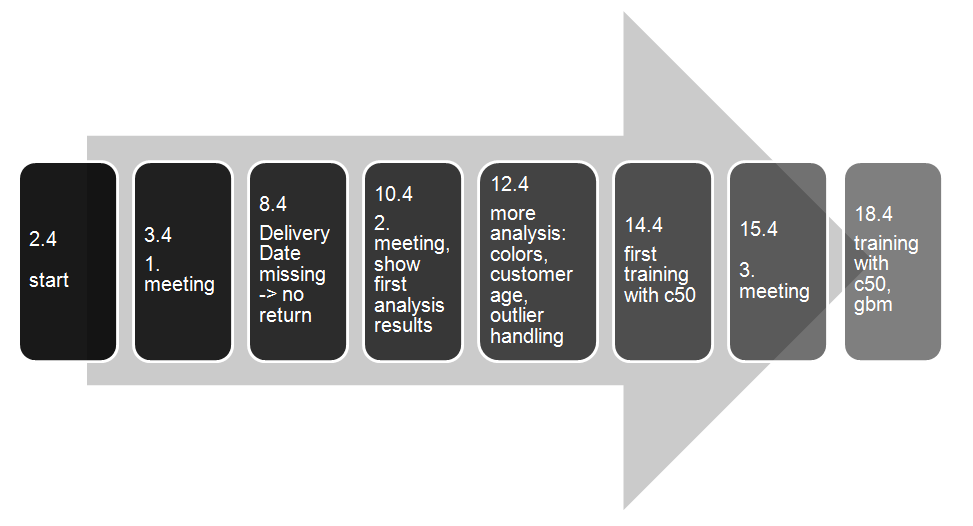
\includegraphics[scale=0.45]{timeline1.png}
\end{frame}

\begin{frame}
\frametitle{Timeline}
	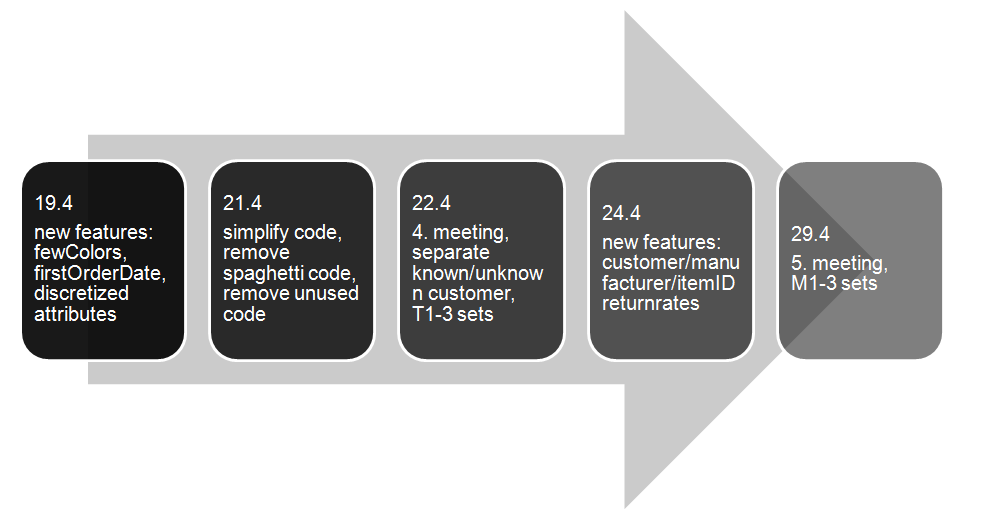
\includegraphics[scale=0.45]{timeline2.png}
\end{frame}

\begin{frame}
\frametitle{Timeline}
	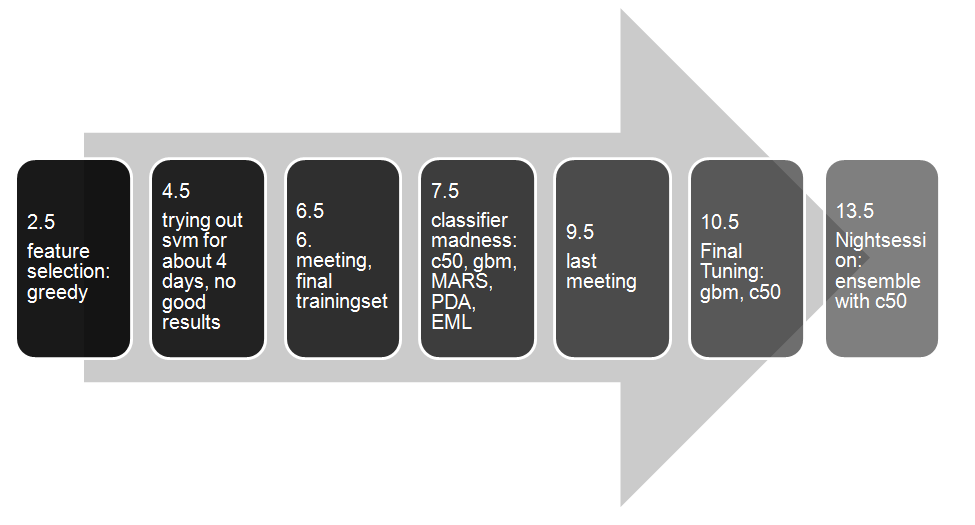
\includegraphics[scale=0.45]{timeline3.png}
\end{frame}


\begin{frame}
\frametitle{Tuning - Parameters}
	\begin{itemize}
	\item C5.0
	\begin{itemize}
		\item model: rules / tree
		\item winnow: true / false
		\item trials: int
	\end{itemize}
	\item Stochastic Gradient Boosting
	\begin{itemize}
		\item shrinkage: double
		\item trees: int
		\item interactiondepth: int
	\end{itemize}
	\item For both: more parametertuning possible
	\end{itemize}
\end{frame}

\begin{frame}
\frametitle{Tuning - Theory}
	\begin{itemize}
	\item C5.0
	\begin{itemize}
		\item more trials $\rightarrow$ better
		\item winnowing $\rightarrow$ depends
		\item rules $\rightarrow$ takes more time (conversion after learning step)
	\end{itemize}
	\item Stochastic Gradient Boosting
	\begin{itemize}
		\item shrinkage $\rightarrow$ less = better
		\item problem: less shrinkage needs more trees to be good
		\item trees $\rightarrow$ more = better
		\item interactiondepth $\rightarrow$ depends
	\end{itemize}
	\end{itemize}
\end{frame}

\begin{frame}
\frametitle{Tuning - Practice in DMC}
	\begin{itemize}
	\item C5.0
	\begin{itemize}
		\item more trials $\rightarrow$ better
		\item computing time increases linearly, not worth it beyond 100 trials
		\item less than 100 trials $\rightarrow$ rules better, else tree
		\item overall accuracy increase: about 0,5\%
	\end{itemize}
	\item Stochastic Gradient Boosting
	\begin{itemize}
		\item shrinkage $\rightarrow$ 0.001 minimum, more not computable in time
		\item trees $\rightarrow$ around 300
		\item interactiondepth $\rightarrow$ 5-7
		\item overall accuracy increase: about 1\%
	\end{itemize}
	\item For both: more parametertuning possible
	\end{itemize}
\end{frame}

\end{document}